


{  \setbeamercolor{background canvas}{bg=sectioncolor}
\begin{frame}{RTE Representation: Challenge \textnumero 1}

  How to represent an RTE in Scala?


  \medskip
  
  \begin{itemize}
  \item Surface syntax: declarative, expressive, composable
  \item Programmatic interface: reflective, algebraic manipulation
  \item Library: \code{rte}
  \end{itemize}
\end{frame}
}

\newsavebox\exnotebox
\begin{lrbox}{\exnotebox}
  \begin{minipage}{6.5cm}
    %% dont re-indent this file
\begin{lstlisting}[style=scalaioScala]
val I:Rte = Atomic(classOf[Int])
val F:Rte = Atomic(classOf[Float])
val D:Rte = Atomic(classOf[Double])

val re:Rte = (I ++ (D | F).+).*
\end{lstlisting}

  \end{minipage}
\end{lrbox}


\begin{frame}{RTEs}{What are Regular Type Expressions?}
  \begin{columns}
    \begin{column}{0.55\textwidth}
  \begin{itemize}
  \item Mathematical notation: $(Int \cdot (Double \cup Float)^+)^*$
  \item Scala notation\\
    \usebox\exnotebox
  \item Leaf nodes interface to Scala Type System
  \end{itemize}
    \end{column}%
    \begin{column}{0.45\textwidth}
      \scalebox{0.7}{% Modeled after the following
% A simple Tree
% Author: Stefan Kottwitz
% https://www.packtpub.com/hardware-and-creative/latex-cookbook
\documentclass[border=10pt]{standalone}
\usepackage{tikz}
\begin{document}
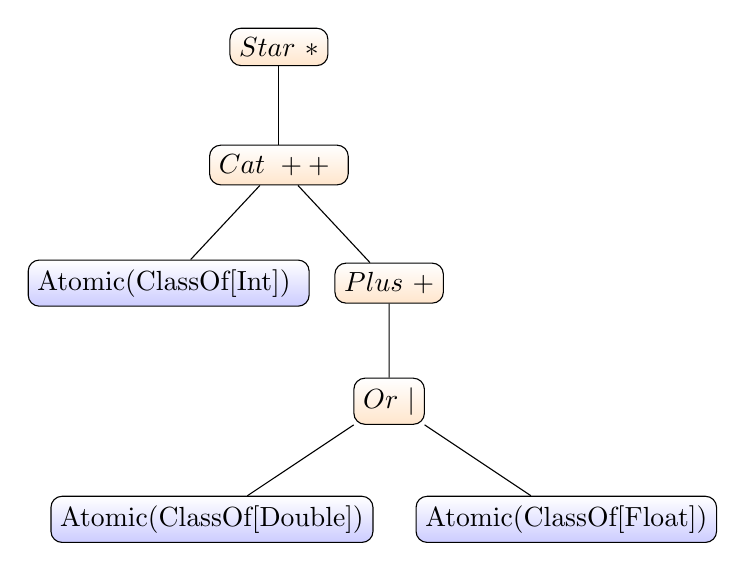
\begin{tikzpicture}[sibling distance=10em,
  every node/.style = {shape=rectangle, rounded corners,
    draw, align=center,
    top color=white, bottom color=orange!20}]]
    \tikzstyle{level 2}=[sibling distance=28mm]
    \tikzstyle{level 4}=[sibling distance=45mm]
  \node {$Star~*$}
  child { node { $Cat~++$ } 
    child { node [bottom color=blue!20] {\text{Atomic(ClassOf[Int])} }}
    child { node {$Plus~+$} 
      child { node {$Or~|$}
        child { node [bottom color=blue!20] {\text{Atomic(ClassOf[Double])}} }
        child { node [bottom color=blue!20] {\text{Atomic(ClassOf[Float])}} } } } } ;
\end{tikzpicture}
\end{document}
}
    \end{column}%
  \end{columns}%
\end{frame}


\newsavebox\exampleAbox
\begin{lrbox}{\exampleAbox}
  \begin{minipage}{12cm}
    %% dont re-indent this file
\begin{lstlisting}[style=scalaioScala]
val data = Seq("C", 100, 200, 300,
               "M", 10.0, 20.0,
               "M",
               "C", 1, 2, 3,
               "C", -1, -3, -7, -8)
\end{lstlisting}

  \end{minipage}
\end{lrbox}



\begin{frame}{Example 2}{An RTE to match}
  \usebox\exampleAbox

  \begin{itemize}
  \item Keyword strings \code{"C"} (counts) and \code{"M"} (measurements)
  \item \code{"C"} followed by zero or more \code{Int} values
  \item \code{"M"} followed by zero or more values, \code{Double} or \code{Float}
  \end{itemize}
\end{frame}

\newsavebox\exampleAbbox
\begin{lrbox}{\exampleAbbox}
  \begin{minipage}{12cm}
    %% dont re-indent this file
\begin{lstlisting}[style=scalaioScala]
val data = Seq("C", 100, 200, 300, // count
                 "M", 10.0, 20.0, // measurement
                 "M",
                 "C", 1, 2, 3,
                 "C", 1, 3, 7, 8)

val F:Rte = Atomic(classOf[Double]) | Atomic(classOf[Float])
val I:Rte = Atomic(classOf[Int])
val keyM:Rte = Eql("M")
val keyC:Rte = Eql("C")

val re:Rte = ((keyC ++ I.*) | (keyM ++ F.*)).*

re.contains(data) // returns true
\end{lstlisting}

  \end{minipage}
\end{lrbox}



\begin{frame}{Example 2}{Successful match}
  \usebox\exampleAbbox
\end{frame}

\newsavebox\exampleAcbox
\begin{lrbox}{\exampleAcbox}
  \begin{minipage}{12cm}
    %% dont re-indent this file
\begin{lstlisting}[style=scalaioScala]
val bad   = Seq("C", 100, 200, 300,
                 "M", 10.0, 20.0,
                 "M",
                 "C", 1, ~~2.0~~, 3, // VIOLATES PATTERN
                 "C", 1, 3, 7, 8)

val F:Rte = Atomic(classOf[Double]) | Atomic(classOf[Float])
val I:Rte = Atomic(classOf[Int])
val keyM:Rte = Eql("M")
val keyC:Rte = Eql("C")

val re:Rte = ((keyC ++ I.*) | (keyM ++ F.*)).*

re.contains(~~bad~~) // returns false
\end{lstlisting}

  \end{minipage}
\end{lrbox}



\begin{frame}{Example 2}{Does not match}
  \usebox\exampleAcbox
\end{frame}

\newsavebox\exampleAdbox
\begin{lrbox}{\exampleAdbox}
  \begin{minipage}{12cm}
    %% dont re-indent this file
\begin{lstlisting}[style=scalaioScala]
val F:Rte = Atomic(classOf[Double]) | Atomic(classOf[Float])
val I:Rte = Atomic(classOf[Int])
val keyM:Rte = Eql("C")
val keyC:Rte = Eql("M")

val re:Rte = ((keyC ++ I.*) | (keyM ++ F.*)).*
\end{lstlisting}

  \end{minipage}
\end{lrbox}


%% \begin{frame}{Example 2}{DFA}
%%   \usebox\exampleAdbox
  
%%   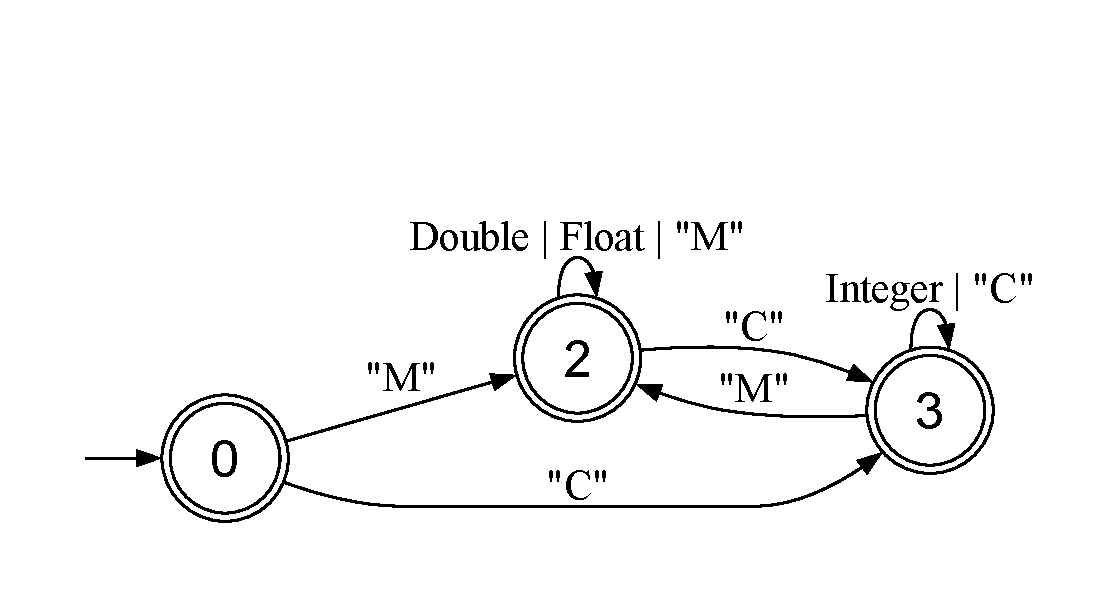
\includegraphics[height=0.5\textheight,trim = {1.8cm 1.0cm 0 3.5cm}, clip]{example2.pdf}
%% \end{frame}


%% \newsavebox\rteast
%% \begin{lrbox}{\rteast}
%%   \begin{minipage}{11cm}
%%     %% dont re-indent this file
\begin{lstlisting}[style=scalaioScala]
val Int:Rte      = Atomic(classOf[Int])
val Double:Rte   = Atomic(classOf[Double])
val Float:Rte    = Atomic(classOf[Float])

val re:Rte = Int ++ (Double | Float).*
\end{lstlisting}

%%   \end{minipage}
%% \end{lrbox}


%% \begin{frame}{Example RTE Expression Tree}
%%   \begin{columns}[T]
%%     \begin{column}{0.55\textwidth}
%%       \usebox\rteast
%%     \end{column}%
%%     \begin{column}{0.45\textwidth}
%%       \scalebox{0.7}{% Modeled after the following
% A simple Tree
% Author: Stefan Kottwitz
% https://www.packtpub.com/hardware-and-creative/latex-cookbook
\documentclass[border=10pt]{standalone}
\usepackage{tikz}
\begin{document}
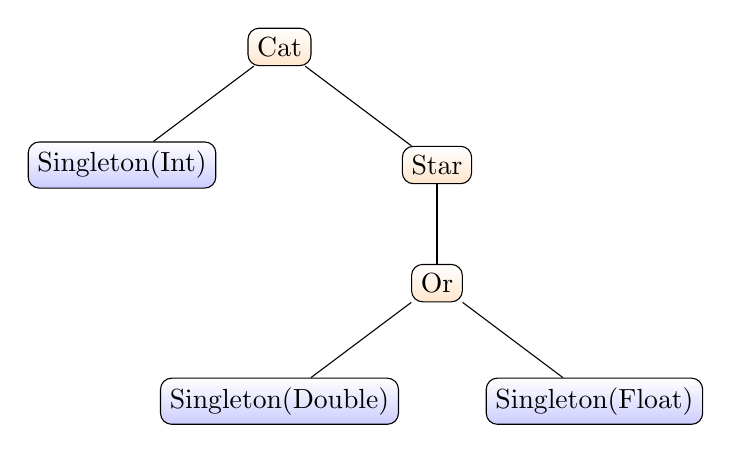
\begin{tikzpicture}[sibling distance=10em,
  every node/.style = {shape=rectangle, rounded corners,
    draw, align=center,
    top color=white, bottom color=orange!20}]]
    \tikzstyle{level 1}=[sibling distance=40mm]
    \tikzstyle{level 2}=[sibling distance=80mm]
    \tikzstyle{level 3}=[sibling distance=40mm]
  \node {Cat}
    child { node [bottom color=blue!20] {Singleton(Int)}}
    child { node {Star}
      child { node {Or} 
        child { node [bottom color=blue!20] {Singleton(Double)} }
        child { node [bottom color=blue!20] {Singleton(Float)} } } } ;
\end{tikzpicture}
\end{document}
}
%%     \end{column}
%%   \end{columns} 
  
%%   \medskip
  
%%   \begin{itemize}
%%   \item An RTE is an expression tree (abstract syntax
%%     tree, AST),
%%   \item Each node is an instance of class \code{Rte}.
%%   \item Leaf nodes interface to Scala classes via \code{Atomic(...)}.
%%   \end{itemize}
%% \end{frame}

\begin{frame}{\code{Rte} class quasi-ADT}
  \scalebox{0.9}{% Modeled after the following
% A simple Tree
% Author: Stefan Kottwitz
% https://www.packtpub.com/hardware-and-creative/latex-cookbook
\documentclass[border=10pt]{standalone}
\usepackage{tikz}
\begin{document}
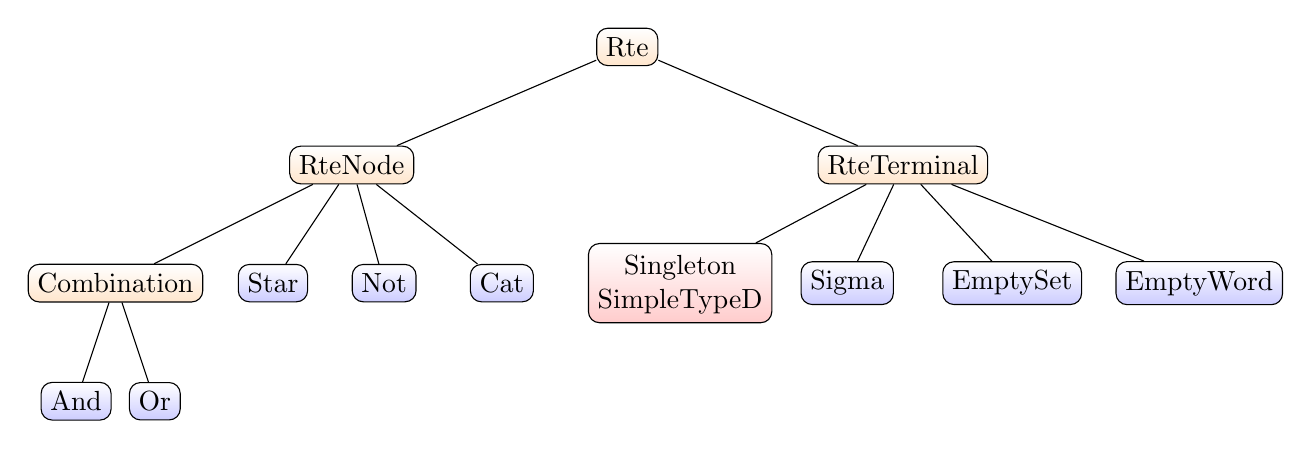
\begin{tikzpicture}[sibling distance=10em,
  every node/.style = {shape=rectangle, rounded corners,
    draw, align=center,
    top color=white, bottom color=blue!20}]]
    \tikzstyle{level 1}=[sibling distance=70mm]
    \tikzstyle{level 2}=[sibling distance=20mm]
    \tikzstyle{level 3}=[sibling distance=10mm]
  \node [bottom color=orange!20] {Rte}
    child { node [bottom color=orange!20] {RteNode}
      child { node [bottom color=orange!20] {Combination} 
        child { node {And} }
        child { node {Or} } }
      child { node {Star} }
      child { node [right=-10mm] {Not} }
      child { node [right=-15mm] {Cat} } }
    child { node [bottom color=orange!20] {RteTerminal}
      child { node [text height=20pt, right=-10mm, top color=white, bottom color=red!20] {Singleton\\SimpleTypeD} }
      child { node [right=-3mm] {Sigma} }
      child { node [right=-5mm] {EmptySet} }
      child { node [right=-3mm] {EmptyWord} } } ;
\end{tikzpicture}
\end{document}
}

  \medskip

  \begin{itemize}
  \item RTE nodes (and leafs) defined by the class hierarchy \code{Rte}
  \item The \code{Singleton} class interfaces to the type system.
  \item \code{SimpleTypeD} is an abstraction of Scala/Java class (later)
  \item Not an ADT for a \Emph{silly} reason, (single file  \code{sealed} classes).
  \end{itemize}
\end{frame}

%% \newsavebox\leafbox
%% \begin{lrbox}{\leafbox}
%%   \begin{minipage}{12cm}
%%     %% dont re-indent this file
\begin{lstlisting}[style=scalaioScala]
EmpySet   // empty set of sequences.
Sigma     // singleton sequences.
EmptyWord // empty sequences.

// singleton sequences of Int and of String
val Int:Rte = Atomic(classOf[Int])    
val Str:Rte = Atomic(classOf[String])

Int.contains(List(42))      // returns true
Int.contains(List("hello")) // returns false
Str.contains(List("hello")) // returns true
Str.contains(List())        // returns true
\end{lstlisting}

%%   \end{minipage}
%% \end{lrbox}

%% \begin{frame}{\code{Rte} subclasses}{Terminal}
%%   \usebox\leafbox
%% \end{frame}

%% \newsavebox\orbox
%% \begin{lrbox}{\orbox}
%%   \begin{minipage}{12cm}
%%     %% dont re-indent this file
\begin{lstlisting}[style=scalaioScala]
val r1:Rte = Or(EmptySeq, Int, Str)
val re:Rte = EmptySeq | Int | Str
      
re.contains(List(42)) // returns true
re.contains(List("hello")) // returns true
re.contains(List(42, "hello")) // returns false
\end{lstlisting}

%%   \end{minipage}
%% \end{lrbox}

%% \newsavebox\andbox
%% \begin{lrbox}{\andbox}
%%   \begin{minipage}{12cm}
%%     %% dont re-indent this file
\begin{lstlisting}[style=scalaioScala]
val re:Rte = And(Int.*, Odd ++ Sigma.* ++ Even)
      
re.contains(List(41,42)) // returns true
re.contains(List(1,2,3,4)) // returns true
re.contains(List(42, "hello")) // returns false

// intersection, Demorgan's equality
assert( r1 & r2 == !(!r1 | !r2)) // for all r1, r2
\end{lstlisting}

%%   \end{minipage}
%% \end{lrbox}


%% \begin{frame}{\code{Rte} subclasses}{Union, Or}
%%   \usebox\orbox
%%  \end{frame}




%% \newsavebox\catbox
%% \begin{lrbox}{\catbox}
%%   \begin{minipage}{12cm}
%%     \begin{lstlisting}[style=scalaioScala]
val r1:Rte = EmptyWord | Int | str
val r2:Rte = Cat(Int, Str, r1)
val r2:Rte = Int ++ str ++ r1

r2.contains(List(42, "hello")) // returns true
r2.contains(List(42, "hello", 42)) // returns true
r2.contains(List("hello", 42)) // returns false
\end{lstlisting}

%%   \end{minipage}
%% \end{lrbox}


%% \begin{frame}{\code{Rte} subclasses}{Concatenation}
%%   \usebox\catbox
%%  \end{frame}



%% \newsavebox\starbox
%% \begin{lrbox}{\starbox}
%%   \begin{minipage}{12cm}
%%     %% dont re-indent this file
\begin{lstlisting}[style=scalaioScala]
val r3:Rte = Star(Int) // or Int.*
r3.contains(List(1,2,3,4,5)) // returns true

val r4:Rte = Star(Str) // or Str.*
r4.contains(List("a", "b", "c")) // returns true
r4.contains(List(1, "hello", 2, 3, "world") // return false

val r5:Rte = Star(Int | Str) 
r5.contains(List(1, "hello", 2, 3, "world") // return true
\end{lstlisting}

%%   \end{minipage}
%% \end{lrbox}

%% \newsavebox\notbox
%% \begin{lrbox}{\notbox}
%%   \begin{minipage}{12cm}
%%     %% dont re-indent this file
\begin{lstlisting}[style=scalaioScala]
val re:Rte = Not(Int) // or !Int

re.contains(List(1)) // returns false
re.contains(List(1,2)) // returns true
re.contains(List("hello")) // returns true
\end{lstlisting}

%%   \end{minipage}
%% \end{lrbox}


%% \begin{frame}{\code{Rte} subclasses}{Repetition, Kleene Star}
%%   \usebox\starbox
%% \end{frame}

%% \begin{frame}{\code{Rte} subclasses}{Inversion, Not}
%%   \usebox\notbox

%%   \bigskip

%%   Matches any sequence other than what is matched by a given \code{re}.
%% \end{frame}

%% \begin{frame}{\code{Rte} subclasses}{Intersection, And}
%%   \usebox\andbox
%%  \end{frame}


\newsavebox\extendedbox
\begin{lrbox}{\extendedbox}
  \begin{minipage}{12cm}
  %% dont re-indent this file
\begin{lstlisting}[style=scalaioScala]
// binary infix operators
r1 & r2 == And(r1,r2)
r1 | r2 == Or(r1,r2)
r1 ++ r2 == Cat(r1,r2)

// complement (unary)
!re == Not(re)

// one/zero or more, optional
re.* == Star(re)
re.+ == re ++ re.*
re.? == EmptySeq | re

// exponent, n-times
re^4 == re ++ re ++ re ++ re
\end{lstlisting}

  \end{minipage}
\end{lrbox}

\begin{frame}{Extended RTEs}{Some Syntax Sugar}
  \usebox\extendedbox
\end{frame}
